
\documentclass[12pt]{article}
\usepackage[utf8]{ inputenc}
\usepackage[brazil]{babel}
\usepackage{hyperref}
\usepackage{graphicx}
\usepackage{geometry}
\geometry{left=2.5cm,right=2.5cm,top=2.5cm,bottom=2.5cm}
\graphicspath{{../../imagens/capitulo4/}}
%----------------------------------------------------------
\hypersetup{
    colorlinks=true,
    linkcolor=blue,
    filecolor=magenta,
    urlcolor=cyan,
}
%----------------------------------------------------------
\title{\textbf{LDO - Capítulo 4\\
Tópicos de Machine Learning}}

\author{Igor Marques Reis}
\date{23/10/2020}
%----------------------------------------------------------
\begin{document}
    \maketitle

    \centering Agora que você já tem uma visão mais ampla sobre Machine Learning,
que tal pesquisar um pouco sobre as situações em que ela pode ser
utilizada, e muitas vezes, \href{https://www.deal.com.br/blog/7-maneiras-de-como-a-inteligencia-artificial-esta-mudando-nosso-dia-a-dia/}{mudar a vida das pessoas}?


    \centering \large\textbf{Vamos lá!}
    
%---------------------------   texto 1
            \section*{\centering Machine Learning na educação:}\label{sec:ML_Na_Educacao}
            
            \begin{figure}[ht]
            \centering
            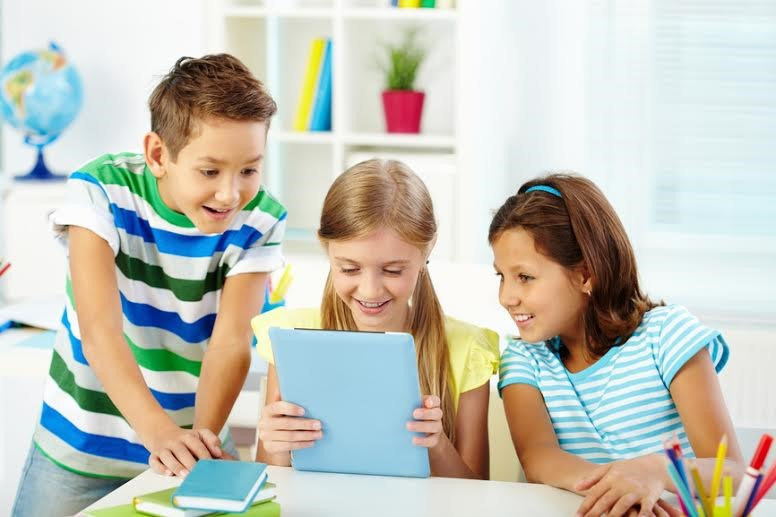
\includegraphics[scale=0.4]{ldo-1.jpg}               
            \end{figure}
            
    Sabemos que não é novidade para ninguém que os smartphones e seus aplicativos já
fazem parte do processo de educação, inclusive há instituições de ensino que utilizam ativamente
essas ferramentas para auxiliar o processo de aprendizagem de seus alunos.
Já pensou em ter um professor que está sempre disponível para tirar
suas dúvidas, e tudo você precisa fazer para contatá-lo seria abrir um
app no seu celular? Se você achou isso interessante, recomendo
assistir a \href{https://www.youtube.com/watch?v=Gjm1xgJVij4}{esse vídeo}!\\

Legal, né? Mas ainda não acabou... se você gosta de
videogames, provavelmente o próximo tópico vai chamar sua atenção.
%---------------------------   texto 2 
           \section*{\centering \textbf{Conheça o MarI/O:}}\label{sec:MarI/O}
\

\

Se você não jogou, tenho certeza que pelo menos já ouviu falar sobre o
jogo Super Mario ou qualquer outro dessa extensa franquia, certo?
Já pensou poder completar aquele nível difícil, ou então até mesmo
passar de uma fase que você já passou antes, mas esqueceu de
salvar?

\

\


            \begin{figure}[ht]
            \label{fig:classificação}
            \centering
            
\includegraphics[scale=0.3]{ldo-2.jpg}               
            \end{figure}
            
\

\


A princípio, \href{https://www.youtube.com/watch?v=qv6UVOQ0F44}{esse vídeo} pode parecer como qualquer outro gameplay de Super Mario, até você saber que, na verdade, quem está jogando é uma
máquina! Isso mesmo! \href{https://www.youtube.com/channel/UC8aG3LDTDwNR1UQhSn9uVrw}{O criador} desse projeto – denominado MarI/O –
criou todo o aprendizado de máquina do ZERO. De acordo com ele,
quando começou o projeto, o “jogador” não sabia nem o que era Super
Mario, muito menos andar para a direita (o que é essencial em jogos de
plataforma). Através de técnicas de aprendizado de máquina ele
conseguiu fazer com que as fases do jogo sejam completadas com
perfeição (sem nenhuma morte!). Incrível, né?
           
%---------------------------   texto 3
           \clearpage
           \section*{\centering Machine Learning em negócios:}\label{sec:ML_Negocios}
           \begin{figure}[ht]
           \centering
           
\includegraphics[scale=0.5]{ldo-3.1.png}
           \end{figure}
   
           Já pensou em fundar uma empresa? Ser seu próprio chefe? Saiba que
o Machine Learning pode te ajudar nessa empreitada! Já pensou em
conseguir identificar os níveis de risco e estimar o tempo de retorno de
um investimento como esse?
            
            \paragraph{}
           \begin{figure}[ht]
           \centering
           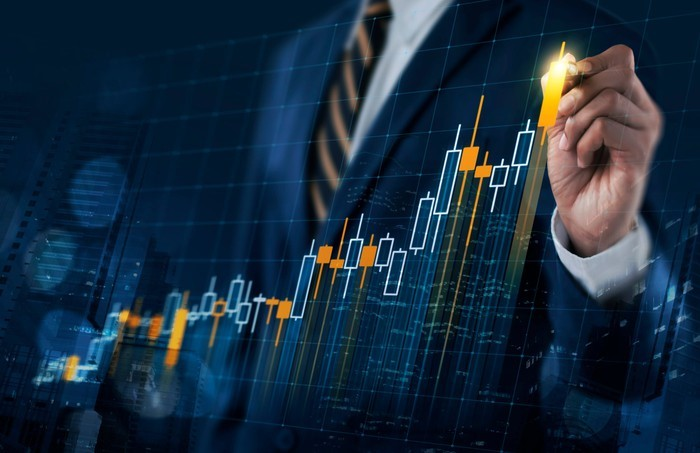
\includegraphics[scale=0.5]{ldo-3.2.jpg}
           \end{figure}
           
           Entender melhor o cliente e suas necessidades, melhorar a eficiência no
marketing? \href{https://forbes.com.br/negocios/2019/09/15-maneiras-como-o-machine-learnings-ajuda-nos-negocios/#foto11}{Tudo isso e muito mais} pode ser auxiliado com o
aprendizado de máquina. Fundar e, principalmente, manter uma
empresa é extremamente trabalhoso e consome muito tempo, então
qualquer ajuda (\href{https://epocanegocios.globo.com/Tecnologia/noticia/2019/02/startup-usa-ciencia-de-dados-para-prever-o-futuro-das-empresas-e-ajuda-las-lucrar-mais.html}{desde que seja boa}) é muito válida!

%---------------------------   Extras
        
            \section*{\centering Material extra/Referências:}\label{sec:Extra_Referencias}

\
           
            \begin{itemize}
            
            %---------------------------------------
                \item
                \href{https://itforum.com.br/colunas/como-o-machine-learning-e-a-ia-podem-revolucionar-a-educacao/}{Como o machine learning e a IA podem revolucionar a educação.}

            
            %----------------------------------------    
                \item
                \href{https://cer.sebrae.com.br/machine-learning-na-educacao-como-funciona/}{Machine Learning na educação: Como funciona?}

            
            %----------------------------------------
             \item
             \href{https://machinelearningforkids.co.uk/?lang=pt-br#!/about}{Machine Learning para crianças.
}
            
            %----------------------------------------
             \item   
             \href{https://medium.com/machina-sapiens/aprendizagem-de-m\%C3\%A1quina-\%C3\%A9-divertido-parte-2-7c00d034e1d5}{ Usando Aprendizagem de Máquina para gerar níveis de Super Mario}
            
            %----------------------------------------
             \item
             \href{https://paulovasconcellos.com.br/explicando-deep-reinforcement-learning-com-super-mario-ao-inv\%C3\%A9s-de-matem\%C3\%A1tica-4c77392cc733}{Deep Reinforcement Learning com Super Mario}: Uma introdução simples para quem não tem paciência para fórmulas.
             
             %----------------------------------------
             \item  
             \href{https://minerandodados.com.br/diferentes-utilizacoes-de-machine-learning-no-mercado-financeiro/}{Diferentes Utilizações de Machine Learning no Mercado Financeiro.}
             
             %----------------------------------------
             \item 
             \href{http://bibliotecadigital.fgv.br/dspace/bitstream/handle/10438/27999/carolina_calio_nogueira_VF.pdf?sequence=1&isAllowed=y}{Dissertação de mestrado} que estuda o uso de Machine Learning para prever o mercado de ações.
             
            \end{itemize}

        
          

        
\end{document}